\documentclass[conference]{IEEEtran}

\pagestyle{plain}

\usepackage[utf8]{inputenc}
\usepackage{graphicx}
\usepackage{xcolor}
\usepackage{svg}
\usepackage{booktabs}
\usepackage{multirow}
\usepackage{amsmath}
\usepackage{algpseudocode}
\usepackage{listings}
\usepackage{subcaption}
\usepackage{comment}
\usepackage[hidelinks]{hyperref}
\usepackage[T1]{fontenc}
%\usepackage{lmodern} % TODO: work out why this doesn't compile without this https://tex.stackexchange.com/questions/10706/pdftex-error-font-expansion-auto-expansion-is-only-possible-with-scalable
\lstset{
  basicstyle=\ttfamily,
  columns=fullflexible,
  frame=single,
  breaklines=true,
  tabsize=4,
}

\newcommand{\red}[1]{\textcolor{red}{#1}}
\newcommand{\redcomment}[1]{\textcolor{red}{(#1)}}

\begin{document}

\title{Satellite Spoofing from A to Z: On the Requirements of Satellite Overshadowing Attacks}
\author{Anonymous Authors}

\begin{comment}
\author{\IEEEauthorblockN{Edd Salkield}
\IEEEauthorblockA{University of Oxford\\
edd.salkield@cs.ox.ac.uk}
\and
\IEEEauthorblockN{Joshua Smailes}
\IEEEauthorblockA{University of Oxford\\
joshua.smailes@cs.ox.ac.uk}
\and
\IEEEauthorblockN{Richard Baker}
\IEEEauthorblockA{University of Oxford\\
richard.baker@cs.ox.ac.uk}
\and
\IEEEauthorblockN{Martin Strohmeier}
\IEEEauthorblockA{Cyber-Defence Campus, armasuisse Science + Technology\\
martin.strohmeier@armasuisse.ch}
\and
\IEEEauthorblockN{Ivan Martinovic}
\IEEEauthorblockA{University of Oxford\\
ivan.martinovic@cs.ox.ac.uk}}
\end{comment}

\IEEEoverridecommandlockouts
\makeatletter\def\@IEEEpubidpullup{6.5\baselineskip}\makeatother
\IEEEpubid{\parbox{\columnwidth}{
    Network and Distributed System Security (NDSS) Symposium 2023\\
    28 February - 4 March 2023, San Diego, CA, USA\\
    ISBN 1-891562-83-5\\
    https://dx.doi.org/10.14722/ndss.2023.23xxx\\
    www.ndss-symposium.org
}
\hspace{\columnsep}\makebox[\columnwidth]{}}

\maketitle

\begin{abstract}
Data from Earth-observing satellites has become crucial in private enterprises, research applications, and in coordinating national responses to events such as forest fires.
These purposes are supported by datasets derived from a variety of satellites, some of which were launched decades ago.
Since then, attitudes to securing the physical layer have changed, opening the door for modern adversaries to overshadow the signal with commercially available radio equipment.

In this paper, we consider how this leads to poisoning satellite-derived datasets and exploiting the processing systems themselves.
As a case study, we consider NASA's live forest fire detection system, which is sent to users in more than 160 countries.
We demonstrate that the attacker can arbitrarily manipulate fires in the derived dataset to trigger false emergency response or mislead crisis analysis, and achieve denial of service and code execution in the processing software.
Through radio simulation, we show that the required signal overshadowing can be achieved by a terrestrial attacker despite the highly directional nature of the dish.
This raises concerns that any dataset derived from these satellites could be compromised by similar means.
\end{abstract}


\section{Motivation}

Satellite-derived data has become a key part of critical infrastructure for private, national, and scientific use.
Although new satellites are being launched at a high rate, even decades-old satellites are seeing novel use cases including advanced forest fire detection~\cite{nasaFirms} and analysing separatist-controlled regions during recent conflicts~\cite{separatistLuminosity}. % TODO: cite a new forest fire paper, not FIRMS
These systems were built when robust cryptography was uncommon due to less powerful onboard computers.
It is now well accepted that legacy software which handle data with little-to-no authentication, such as these terrestrial processing systems, are not resilient against modern adversaries.
However, this was not a practical concern at the time since attacks at the physical layer would have required a costly and highly specialized setup.
Consequently, there does not exist any current work to understand the effects of a modern adversary against such a system.

Nowadays, software-defined radio hardware, capable of emitting arbitrarily encoded signals at the correct frequency, is readily available off the shelf.
This lowers the barrier to entry for signal injection attacks significantly.
Accordingly, both existing and novel use cases must now contend with the effects of signal injection, which include poisoning the dataset and exploiting the decoder.
This has far-reaching ramifications due to increased reliance on satellite-derived datasets.

% Expand on in what way satellites are key infrastructure
    % Maybe mention EOS fleet
% how was setup specialised for previous attackers. Evidence for this?
% Existing systems that weren't resilient against modern adversaries, and the benefits of reviewing them
% Justifying how SDRs are more available, and looking at the estimated cost of pulling off the attack

As global reliance on on satellite data increases, the security implications are becoming increasingly relevant.
Recent news demonstrates that motivated adversaries do in fact exist, and are interested in exploiting the decoding and demodulating pipelines.
For example, in a recent attack against ViaSat's satellite broadband capability, a side channel terrestrial network permanently disabled the demodulating hardware across Ukraine, coinciding with the Russian invasion~\cite{satcomAnalysis}.

% TODO: narrow down specifically to Earth-observing data
To support a wide range of use cases, raw satellite data is processed into more specialised derived datasets such as for forest fire and storm detection.
This feeds into applications including critical national infrastructure and research-oriented purposes.
The importance of these applications makes attacking the raw data appealing.

These new applications make use of a variety of satellites, some of which were launched decades ago.
Since then radio hardware has become more accessible along with a change in attitudes towards securing data transmissions.
Therefore, both the satellite-derived datasets and the downlink processing systems that create them are potentially vulnerable to signal injection.

The security community is becoming increasingly aware that radio overshadowing in a satellite context has the potential to affect critical services.
As a result, recent countermeasures have been proposed which analyze artifacts of overshadowing on the physical channel to determine the authenticity of the received data.
These artifacts include the timing of the signal~\cite{jedermann2021orbit} and features of the waveform such as unexpected differences in signal-to-noise, amplitude, or others extracted through machine learning techniques~\cite{oligeri2020past}.
However, the impact of signal overshadowing against currently-deployed satellites, and the real-world consequences on the systems that depend upon their data, have not yet been considered.

\subsection{Contributions}

Specifically, we make the following contributions:

\begin{itemize}
    \item We present a systematic review of the impact of a modern adversary against satellite downlink processing systems using attacks at the physical layer;
    \item We analyze the impact of these attacks against FIRMS, NASA's live forest fire detection service, as an end-to-end case study. We demonstrate that overshadowing of the wireless channel is sufficient to arbitrarily manipulate fires detected in the derived dataset, and achieve denial of service and arbitrary code execution on the processing software;
    \item We discuss the potential impact of similar attacks against other satellite-derived datasets, exploring the effects that an attacker could expect to cause in the real world;
    \item We demonstrate the feasibility of radio signal injection using commercial off-the-shelf equipment, taking into account the unique constraints of a terrestrial attacker against a highly directional dish;
    \item We conclude by exploring the applicability of existing countermeasures, with respect to the unique constraints of this context.
\end{itemize}

    % TODO: something about categorising the attacks that are possible?

% Things to mention:
% * Recent satellite hacks, but none really focussing on the downlink system through radio
% * We require a systematisation to analyse the effects that an adversary could have
% * We need to show what real-world systems the attacker could expect to manipulate, so that we can secure them. To do this, we need to follow through a system end-to-end, and extract the general principles.

% * We need realistic simulations at least to tell us what ballpark of cost the attacker needs to expend
% * By manipulating the frame packet header, we can make fires...

% Existing work:
% * We need to follow in the footsteps of existing work which shows that, when similar systems are subjected to scrutiny, practical countermeasures have been proposed which continue to affect the industry as a whole
% Here's how it relates to our work now
% We're aware of the state of the art in other settings

%    Para: The reasons why security wasn't core to the design
%    Para: The ways in which security isn't core
%    Para: The effects of security not being core


\begin{comment}
\textbf{Old motivation below:}


In recent decades, satellite imaging of the Earth's surface has become increasingly important within research and safety-critical contexts alike.
Equipped with optical sensors that can detect a spectrum wider than visible light alone, satellites within NASA's \textit{Earth Observing System} (EOS) fleet have found broad usage within areas such as atmospheric observation, wildfire detection, and deforestation monitoring. \textbf{TODO: cite}
Automated data processing techniques are widely used to provide live data streams for incident response; ensuring data integrity at the radio downlink is therefore of high importance.

Although spoofing attacks have been addressed in recent satellite deployments through the introduction of cryptography, the long lifespans, high associated costs, and backwards compatibility requirements of existing satellite systems have resulted in a resistance towards retrofitting cryptography into these systems.
An additional desire for open data has motivated certain scientific satellite operators, including the EOS fleet operators, to make their data available through public unencrypted broadcast.
Accordingly, several prominent data processing software systems have been developed, which are run at ground stations across the world to receive and decode the transmitted signals, producing indispensable data for near real-time and retrospective Earth monitoring applications.
These processing algorithms are distributed in various ways, with the most popular distribution mechanism being the \textit{International Planetary Observation Processing Package} (IPOPP). %TODO: clarify/justify this claim
IPOPP contains the leading edge EOS satellite decoding algorithms, which have been developed over time by many teams, and are chained together to decode the raw bitstreams into usable data products.

Despite the unauthenticated nature of the data, the processing software found in IPOPP is not built with safety or security in mind -- all received signals are passed through a complex software pipeline designed to decode, process, and store the data to make it useful for later work.
Should an attacker successfully inject their own signal it would be processed by this same system and pass through a wide range of software components, each with their own unique attack surface.

Therefore, through carefully crafting input data, an attacker can target the services which are responsible for decoding each part of the protocol.
For example, the near real-time forest fire alerting services can be targeted through injecting arbitrary image data, causing ficticious alerts or masking legitimate ones.
Malicious packets can also be constructed at the protocol level, which lead to denial of service and arbitrary code execution when processed.
The attack data would be stored in various medium- to long-term storage public storage systems and potentially reprocessed at a later time.

Fixing these security issues is nontrivial due to innate constraints of the satellite hardware, and the complexity of its surrounding software ecoystem.
The attacker has multiple avenues through which to inject data, including through overshadowing the radio signal at receiver stations, and through posting malicious data on the satellite data mailing lists.
It is difficult to fully know the extent to which the system is vulnerable, thanks in part to its distribution mechanism in which large collections of potentially out-of-date software components with active CVEs are bundled.

However, even though achieving theoretical guarantees of data authenticity is impossible without cryptographic primitives, the addition of simple countermeasures and renewed software engineering practises would serve to significantly increase the difficulty of achieving these attacks in a practical setting.

\subsection{Contributions}

In this paper we demonstrate that satellite data processing systems cannot assume that the input data is benign, showcasing the real world dangers associated with this assumption in currently deployed systems.

In Section~\ref{sec:attack}, we demonstrate that through overshadowing the wireless channel with carefully constructed packet data, an attacker can inject arbitrary bytes into targeted processing stages within a decoding pipeline.
This injection provides a gateway to more sophisticated attacks against the specific software implementation of the decoding system.

Using NASA's flagship IPOPP software distribution as a case study, we achieve granular manipulation of the decoded images, denial of service in the near real-time context, and arbitrary code execution on end-user machines during dataset reanalysis.
Both near real-time processing systems and medium- to long-term storage archives are targeted by the malicious payloads, opening up both central systems and end user machines to attack.

% Engineering problems?

We go on to measure the feasibility of these attacks in a real-world setting, taking into account the particular difficulties associated with overshadowing the physical layer encoding phase shift keying in Section~\ref{sec:evaluation}.

We discuss countermeasures in Section~\ref{sec:countermeasures}, considering ways to establish the authenticity of decoded signals using cryptographic and other means.
We consider the benefits of properly implemented cryptography and the constraints required to do so, in addition to discussing situations where deployment of cryptography is impractical or undesirable.
In these situations we show how even simple countermeasures based on timing, waveform, and data-level analysis can significantly increase the difficulty of achieving attacks in a practical context.
Through generalising our approach, we propose scalable countermeasures to permit partial adoption according to an organisation's tolerance for risk.

Finally in Section~\ref{sec:discussion}, we discuss how the practical outworkings of these new risks should affect the security posture within organisations, encompassing a discussion of untrusted user-submitted data and software architecture.
We pay attention to the software architectural principles required to make satellite decoding systems robust against this sort of attack, considering particular issues surrounding legacy software systems.

\end{comment}

\section{Related Work}

% TODO: cite Manulis paper asking for a threat model
% TODO: write about information-theoretic noise model stuff
% TODO: write about GPS in particular, with its spoofing, fingerprinting, countermeasures - basically everything explored, but within this unique context

Security research of the SATCOM link covers eavesdropping, in which messages not intended for public access are decoded by an unauthorised receiver, and signal injection, in which the attacker's messages are inserted into the wireless channel.
Existing eavesdropping research has demonstrated the widespread effectiveness of decoding the messages, given the wide area over which the signals can be received and the lack of robust cryptography on the channel.
However, due to the publicly available specification, lack of cryptography, wide-reaching impact, and a radio frequency within the range of SDRs, GPS has been the focus of SATCOM signal injection and its associated countermeasures.
This work draws upon existing research into signal injection against wireless channels in general, but isn't generalised across different satellite receiver types.

As a result, many of the anti-spoofing countermeasures for SATCOM injection focus on GPS also.
However, certain countermeasures instead depend upon physical-layer characteristics of satellites which generalise beyond GPS.

We proceed to discuss work into eavesdropping, signal injection, and countermeasures in turn.

\subsection{Eavesdropping}

% Basic point: encrypted downlinks are hardly universal
% Unencrypted for many reasons

% TODO: mention existing work in reversing Iridium

Fundamentally, securing communications over a wireless channel requires cryptographic guarantees about data confidentiality, integrity, and authenticity.
Satellite systems are no exception; geostationary satellites in particular can often be received across distances of thousands of kilometers.
As a result, unless the data link is robustly encrypted, anyone with access to suitable radio equipment can receive and decode these transmissions.

Pavur et. al. recently uncovered that since many satellite internet providers do not encrypt the downlink~\cite{pavur2020tale}, passport information of ship crews, aircraft systems, and POS terminal data are all broadcast in the clear.
This advances previous work from 2005 which noted the huge amount of information sent via unsecured satellite broadcast~\cite{adelsbach2005satellite}.
This work also explores the theoretical possibilities of TCP session hijacking by broadcasting signals over a high-speed wired connection.

Cybercriminal gangs have been known to abuse the broadcast property to secretly exfiltrate data; packets sent in the clear to any known satellite customer IP address are receivable anywhere within the satellite's footprint~\cite{satellite_apt}.
Although newer satellite internet providers such as Starlink address this issue, and government agencies are beginning to require encryption~\textbf{TODO: cite}, these legacy systems are still widely used due to long mission lifespans and existing receiver hardware.

Other satellite systems also use insecure downlinks.
For example, several of NASA's the Earth Observing Systems fleet communicate without encryption by design; the data is intended to be open, and so running a custom groundstation is encouraged.
However, since the data is not cryptographically signed, authenticity cannot be verified, opening the door to signal injection attacks.

Additionally, certain satellites that were considered secure at launch are now vulnerable.
For example, the Korean satellite COMS-1 uses single DES encryption~\cite{lrit-key-dec}, which has led to customer keys being successfully extracted from satellite data.
Additionally, the GEO-KOMPSAT-2A satellite had its keys leaked on the Korea Meteorological Administration website, which to this day remain publicly available~\cite{xrit-rx}.

\subsection{Signal injection}

Spoofing attacks are carried out by a variety of methods including replay and forgery in order to fool the receiver into accepting illegitimate messages, and jamming is typically performed using high-power interference.
Other than GPS, the majority of work into signal injection considers non-satellite wireless systems; we touch upon each in turn.

\subsubsection{GPS spoofing}

Signal injection attacks in a GPS context are very well explored.
The requirements for a successful attack within many contexts are well known, including in single- and multi-receiver and multi-attacker contexts~\cite{tippenhauer2011requirements}.
It is also well understood how signal timing and precision affects the success of the attack.

%Much existing work within spoofing and jamming satellite communications focuses on Global Navigation Satellite Systems (GNSS).
%The authors of~\cite{wuSpoofing2020} provide a comprehensive review of known types of spoofing and jamming attacks against these satellites, resulting in incorrectly reported positions and denial of service respectively.


Advances in software-defined radios have opened the door for high-precision GPS spoofing attacks deployable with only cheaply available off-the-shelf hardware~\cite{gps-sdr-sim}.
The communications are surprisingly easy to overshadow, requiring only a simple amplifier and antenna setup due to a number of physical layer factors.
High gain isn't required because the legitimate signal is low power, and is received by an omnidirectional antenna.
The signal is circularly polarized, meaning that the attacker doesn't need to be in phase, as per linear polarisation.
Since the signal is of a sufficiently low frequency, a high frequency upconverter and amplifier is not required, and the signal is not absorbed by objects meaning that line-of-sight is not required.

In GPS, data integrity is often checked on the receiver side, with a so-called GPS Lock.
Once the receiver has locked onto a signal, it rejects signals that cause a vastly deviated distance calculation.
Overcoming this lock therefore requires the attacker generate signals to maintain continuity.
This principle applies in particular to Earth observation data, which is expected to be sampled from a continuous input; systems therefore detect anomalies by looking for large deviations between samples.

%\subsubsection{Non-GPS satellite receivers}

% TODO: scan space attacks open database to check for others

%Outside of a GPS context, the documented signal injection attacks surround satellite television

%Max headroom and similar - TV satellite
%Same protocols as used for satellite internet, traditionally

\subsubsection{Other wireless systems}

Signal injection attacks against the receivers of other wireless systems are also well explored.
These include WiFi, wireless sensors, mobile internet~\cite{yang2019hiding,erni2021adaptover}, GNSS~\cite{tippenhauer2011requirements}, and even avionic systems~\cite{sathayeWireless2019}.

\textbf{TODO: get some advice on this and write it}

Finally, we consider work in physical-layer radio security beyond the scope of satellite communication.
There are a number of deployed radio systems which do not employ cryptography, including the ``ADS-B'' protocol used to locate and track aircraft.
There is a good amount of research into the security of ADS-B: \cite{strohmeierSecurity2015} provides a good review of the extent to which the system is vulnerable and explores ways to make the system more secure through verifying the transmitter location or identity, or using cryptographic methods.
Once again, we can recontextualize a number of these techniques to provide improvements to the security of other unsecured systems, which we see in Section~\ref{sec:countermeasures}.


\subsection{Countermeasures}

As a result, recent countermeasures have been proposed which analyze artifacts of overshadowing on the physical channel to determine the authenticity of the received data~\cite{jedermann2021orbit,oligeri2020past}.
However, the extent to which these countermeasures are effective in preventing overshadowing in a real world setup has yet to be determined.

These methods include consistency checking, measuring signal characteristics, measuring arrival times~\cite{jedermann2021orbit}, utilizing arrays of antennas, measuring angle of signal arrival, and other factors extracted through machine learning techniques~\cite{oligeri2020past}.

\subsubsection{Channel noise masking}

Some information theoretic countermeasures exist, including:

%https://ieeexplore.ieee.org/abstract/document/6739367?casa_token=rwzKea1crRoAAAAA:JYUiN2CdSAzZhFu0jOHq7-d-rINtM_STo4aCzUZasej6ailTUNX4MdaisXcM8G9qvl3AKWk
%https://ieeexplore.ieee.org/abstract/document/6108297?casa_token=hUULRC9BgwgAAAAA:tRxrOhLGzuLjOEE8S7UbXJ_5K4t6QZ0nPRpqiLgmDs7-1okaoezMIb5-HmK-eeCTsL5gcds
%https://ieeexplore.ieee.org/abstract/document/8822950?casa_token=-vLYsKFhvxIAAAAA:P6Xa33aZ_U191d0PGlmW-JdmkoUPYSBQDZ6e2svoM-qonIfm1WLji_smDt-qW1FTc2J2XI8
%https://ieeexplore.ieee.org/document/6638190
%https://ieeexplore.ieee.org/stamp/stamp.jsp?arnumber=6772207&casa_token=NFj6STXZ6mIAAAAA:US_nlhjLLvxy878JkL2F4-JjrgKZoYSH3SpbqwHyFGxbLadVk2foaH4WmccvW_WUe06ZZpc

\subsubsection{Timing analysis}

\subsubsection{Fingerprinting}

\section{Arbitrary Image Injection}

\subsection{Attack description}


Unfortunately the \textit{IPOPP} framework for processing EOS data is open to a variety of attacks through signal injection.
In each case, the attacker leverages different parts of the protocol to redirect the control flow of the program, either causing a denial of service, the leaking of sensitive data, or even arbitrary code execution.

Through the injection of standards-compliant frames, complete with synchronisation headers and checksums, the attacker can convince prior processing stages to decode and demultiplex an arbitrary byte sequence, delivering it as input to \textit{MODISL1DB\_SPA}.

The input to this algorithm is so-called \textit{Level 0} data, which is the body of a data frame with all communications artefacts, including synchronisation headers and checksums, removed.
Through the creation of a custom data frame, the attacker can encapsulate an arbitarary byte sequence which, when overshadowed over the existing signal, will result in the delivery of arbitrary bytes as the input to \textit{MODISL1DB\_SPA}.

We proceed to analyse several classes of attack made possible through this route, and enabled by insecure data handling practises.


\section{Exploiting downlink processing systems}

\subsubsection{Communications interruption}

Downlink satellite communications often take the form of a frame structure, with an easily detectable synchronisation header delimiting them.
An attacker can interrupt the communication through overshadowing a malicious header, causing the state machine to stop decoding the packet and instead resynchronise in the wrong place.

In our analysis, this attack has been shown to be highly effective in preventing

% TODO: insert screenshots side by side of the same signal with overshadowed frame headers

We have analysed the effect of this approach through decoding it through \textit{RT-STPS}.
As \textbf{figure X} shows, this approach is highly effective in denying service.
However, simple signal-to-noise ratio analysis is sufficient to detect that this attack is taking place.

A more stealthy approach can be taken, building upon recent work by Moser et.\ al.  in digital signal cancellation.
Their work has shown that, given bit-perfect knowledge of parts of the signal and the ability to synchronise with it,
phase cancelling from arbitrary distances is possible.
Since the frame header is of a known structure and appears at fixed intervals, this approach would enable the cancellation of the header to below the noise threshold on the receiver, from arbitrary distances.
This approach isn't detectable through signal-to-noise analysis.

\subsubsection{Unprocessable malformed packets}

The software makes assumptions about the internal structure of the packets, which only hold for benign packets.
With the ability to inject arbitrary data, the attacker can craft packets to exploit oversights in the exception handling code for data parsing, and cause the program to crash.
Since the program processes packets in sets, a single malformed packet is sufficient to prevent the processing of the entire set.

Since the packet data is stored as a dataset for future processing, this attack also lets the attacker poison the dataset to make reprocessing of the entire set significantly harder.


\subsubsection{Latent arbitrary code execution}

In addition to near real-time data processing at the downlinks, past data is often reprocessed to take advantage of new processing alorithms, or to explore new results.
To support these use cases, the processing algorithms within MODISL1DB\_SPA are also available as command line tools, with adjustable configurations.

When run in SPA mode, the configuration used is always the same, which has resulted in a "golden path" through the execution of the program which is relatively secure.
However, by changing the initial configuration, a user could accidentally put the program into a mode which unsafely handles the input data.

Therefore, an attacker can poison the official datasets through the injection of packets, which cause no unsafe behaviour on first processing, but leverage vulnerabilities for arbitrary code execution when reprocessed under a different configuration.
These vulnerabilities have the potential to lie dormant in the official data sources as currently distributed by LAADS DAC, among other Direct Readout stations.

% TODO: go on to demonstrate the attack

\subsubsection{Reading unallocated memory}

Due to the design of the hardware on board the satellite, legitimate communications from the onboard instruments are guaranteed to hold to certain assumptions: for example, the packets are always of the same length, and the internal pointers between the packets are always aligned.

However, in this situation it becomes easy to let implicit assumptions about the structure of the data manifest themselves in the data processing.
Code for handling these exceptional cases is often less rigorously tested, because it generally doesn't occur in benign example cases.

However, by providing shorter packets than expected, with larger pointers than expected, we demonstrate how the attacker can take advantage of certain system components written in C to read off the end of the buffer into unallocated memory.
We demonstrate an execution pathway that would result in the resulting data being stored and uploaded to the puclic data archives, theoretically allowing the attacker to leak sensitive information from other processes within the memory of the computer.


\subsubsection{Exploiting bundled dependencies}

In order to make software distribution easier, and to create easily deployable systems that mostly "just work" when extracted into a certain location, the IPOPP algorithms generally come with many bundled dependencies in the source archive.
These files are compiled programs and libraries for the handling of input data, that are intended to work on specific architectures.

However, the practice of bundling libraries with software has long been considered bad from a security perspective, especially since the widespread use of package managers to resolve and install dependencies.
Doing so permits a similar ease of installation, but allows each library and program to be traced back to its dependency, independently updated, and uninstalled when no longer required.

Without a system for managing these dependencies, the system becomes incredibly brittle and hard to change; therefore, there are many dependencies currently present and depended upon that haven't been updated in nearly a decade.
Several of these dependencies have patchable security vulnerabilities for arbitrary code execution, that an attacker could take advantage of.

There are also a large number of dependencies that aren't used for any purpose and are just left around for legacy reasons.
Besides potentially being a risk for privilege escalation, the sheer number of redundant dependencies muddies the water and makes it difficult to discern which depencies need updating as a matter of urgency.

% \begin{itemize}
%     \item Strict separation of data handling code from core program control flow
%     \item Secure distribution and patching of dependencies
%     \item Robustness against configuration changes
% \end{itemize}
 % describe the overall attack structure and hardware setup required
\section{Threat Model}\label{sec:threat-model}

The goal of the adversary is to cause disruption to the EOS image processing pipeline by emitting conterfeit signals in the vicinity of the receiver.
This disruption can take a number of forms:
\begin{itemize}
    \item Inject false data to mislead people -- for example, to disrupt automated systems for forest fire and other anomaly detection,
    \item Mask important data to deny people information -- for instance, to hide approaching natural disasters,
    \item Prevent new data from being processed and saved by the receiver,
    \item Destroy or alter recent or historical data,
    \item Hide malicious payloads in a long-term storage database, to be triggered by a later processing step.
\end{itemize}
%Depending on the scenario, this disruption could take the form of denial of service to the software or hardware components, modification of recently received or historical image data, or destruction of old data.

We assume the attacker has access to commercially available off-the-shelf radio equipment such as Software Defined Radios (SDRs), aplifiers, and antennas, in order to emit signals in the X-band frequency range used by the EOS downlink.
We also assume the attacker is able to maintain a presence in the vicinity of the receiver, in order to inject signals of a sufficient strength that they will be picked up by the receiver.
Crucially, we do not necessarily assume the attacker can emit signals within the beam of the receiving ground station, instead relying on the signal being sufficiently strong that the ground station picks it up regardless of dish orientation.

In order to define realistic price constraints, we consider off-the-shelf radio equipment intended to be used in cubesats.
One cubesat manufacturer, EnduroSat, offers a system capable of encoding and transmitting signals in the X-band for €22,800 and a compatible antenna for €6,400~\cite{endurosat:xbandtransmitter,endurosat:xbandantenna}.
This system has an integrated encoder and is thus not capable of transmitting attacker-crafted sequences of symbols, but it provides us with an understanding of how much similar equipment would cost.
These prices place the attacks within the budget range of a motivated hobbyist, opening the EOS systems up to attacks by a wide range of parties.

We also need to take into account other mechanisms by which the attacker could carry out the intended goals, beyond the scope of the physical layer.
The mailing list for NASA's Direct Readout Laboratory (DRL) provides an attractive entry point -- when a downlink transmission is missed by NASA's ground stations or by another organization, it is routine to use the mailing list to ask someone to send over their own copy of the data~\textbf{TODO cite}.
Our attacker can take advantage of the trust inherent to this system's operation and send over malicious frames, which will be processed without question and entered into the DRL's database.
Of course, it is more difficult to carry out this attack at a specific time due to the ``request/response'' nature of the exchange, but it is still possible to meddle with archived data or attack the processing systems via this method.

Finally, we must consider the sphere of influence of any attacks on the processing systems.
When NASA receives and processes a transmission from a satellite in the EOS fleet, the resulting data is used in a wide range of applications.
We focus on forest fire detection in this paper, but the attacks we describe can easily be adapted to affect other systems connected to the same data streams.
In Section~\ref{sec:background} we review services provided by relying on satellite-derived data; all the services relying on EOS data to provide their services are vulnerable to attacks.

The same is true of any other organisation which processes EOS data, although usually to a lesser extent.
If instead of NASA the attacker targets this organisation's ground station and attached processing system, anything relying on the output data is once again vulnerable.
The distributed nature of ground stations serves to make attacks a little more difficult, but it is still the case that attacking a single ground station affects all datasets derived from data received by that ground station.

Fundamentally, the issue stems from implicit trust of the data source, allowing vulnerabilities to one service to affect any other services further down the processing chain.
\textbf{TODO finish, possibly move further on in the paper}

%The goal of the adversary is to stealthily spoof the image information decoded by a single receiver station by emitting a counterfeit signal in the vicinity of the receiver.  Depending on the scenario, the attacker may want to inject similar-looking images with slight modifications to disrupt automated systems for forest fire and other anomaly detection.  In other cases, the attacker may wish to inject adversarial examples or degrade image quality to harm the research efforts of those using data derived from this source.

%We assume that the attacker has access to off-the-shelf equipment, such as software-defined radios, amplifiers, and antennas.  We also assume that the attacker is able to maintain presence in the vicinity of the images they want to spoof, enabling them to receive the direct broadcast signal for that area [TODO: include roughly how precisely they need to be in the location].  They must also have a presence near the targeted receiver station, and be able to transmit the information they decode between the locations, using systems such as a wired, mobile, or even satellite internet connection.

%We assume that the receiver station has strong waveform and timing analysis on its input signals, utilising state-of-the-art spoofing detection mechanisms.  Although currently few receiver stations perform this analysis, suspicions about the origin of the data may still lead to retrospective analysis.  The attacker must therefore remain stealthy, and manipulate the signal only in ways that still resemble other legitimate signals.

%Finally, the attacker is limited by the physical properties of the radio signal: they are unable to perform the required signal cancellation simply through analogue means, due to the highly limited distance constrains that this requires.  Instead, the attacker must seek to cancel the signal from a distance, requiring that they first receive and process the direct broadcast signal.
\section{Evaluation}\label{sec:evaluation}

\subsection{Data inputs}

\textit{We discuss how an attacker can inject arbitrary bytes into receivers.  We measure the effectiveness of this approach by an overshadowing simulation.  We discuss how data can also be inserted through the mailing list}

\subsection{Security audit}
\textit{Table demonstrating which currently-active CVEs are present in the software. A discussion of legacy software and its relation to security}

\subsection{Physical-Layer Validation}

\begin{figure*}
    \centering
    \begin{subfigure}{0.49\textwidth}
        \centering
        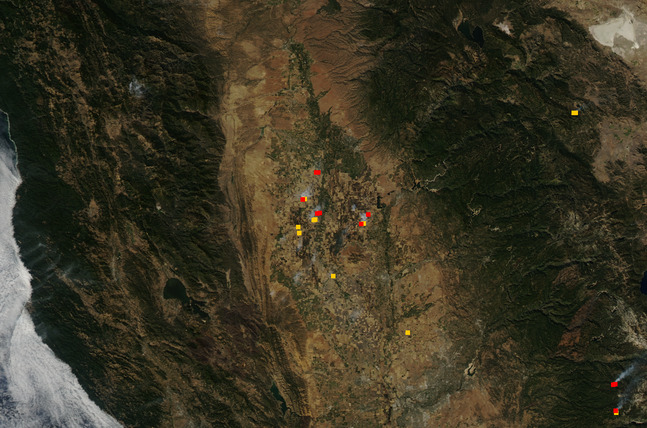
\includegraphics[width=\textwidth]{diagrams/injection/original.jpg}
        \caption{Original image with some fires.}
        \label{fig:injection-orig}
    \end{subfigure}
    \begin{subfigure}{0.49\textwidth}
        \centering
        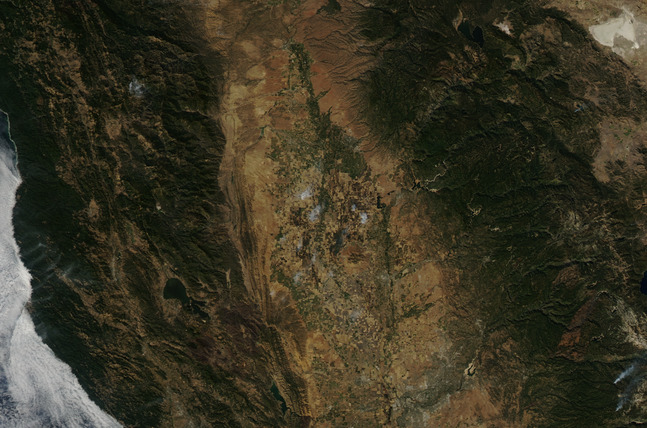
\includegraphics[width=\textwidth]{diagrams/injection/masked_0.jpg}
        \caption{Legitimate fires masked out.}
        \label{fig:injection-masked}
    \end{subfigure}
    \begin{subfigure}{0.49\textwidth}
        \centering
        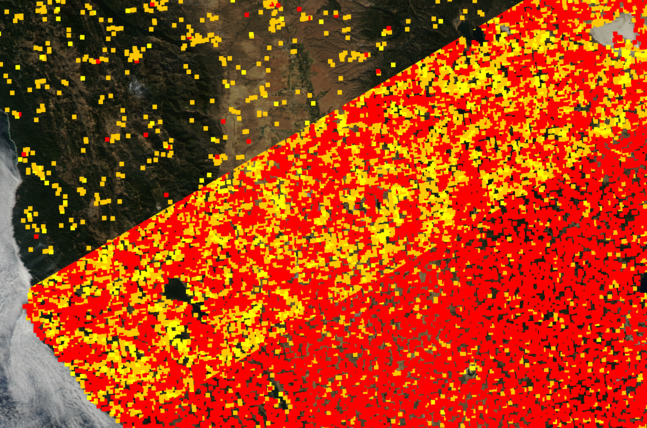
\includegraphics[width=\textwidth]{diagrams/injection/random_combined_diagonal.jpg}
        \caption{Fires randomly injected uniformly across the map. Density and intensity of the fires increases from top to bottom.}
        \label{fig:injection-random}
    \end{subfigure}
    \begin{subfigure}{0.49\textwidth}
        \centering
        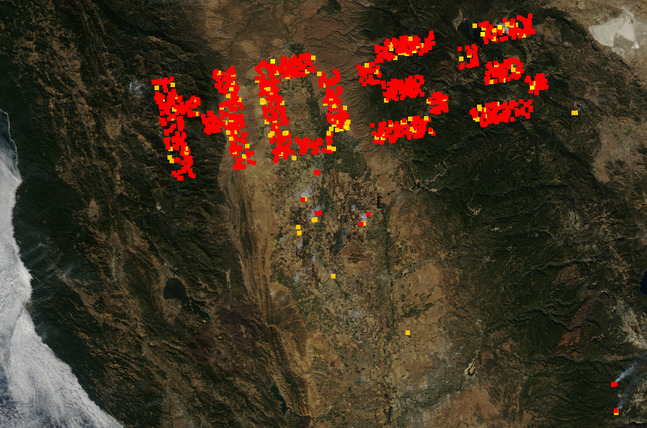
\includegraphics[width=\textwidth]{diagrams/injection/pixels_800_140.jpg}
        \caption{Fires injected at attacker-specified locations.\newline}
        \label{fig:injection-logo}
    \end{subfigure}
    \caption{An overview of the possible ways an attacker can manipulate the output of the forest fire detection algorithm by overshadowing the downlinked data. In each image, forest fires detected by the algorithm are highlighted in yellow, orange, and red in increasing order of intensity.}
    \label{fig:injection}
\end{figure*}

\begin{comment}
\begin{figure}
    \centering
    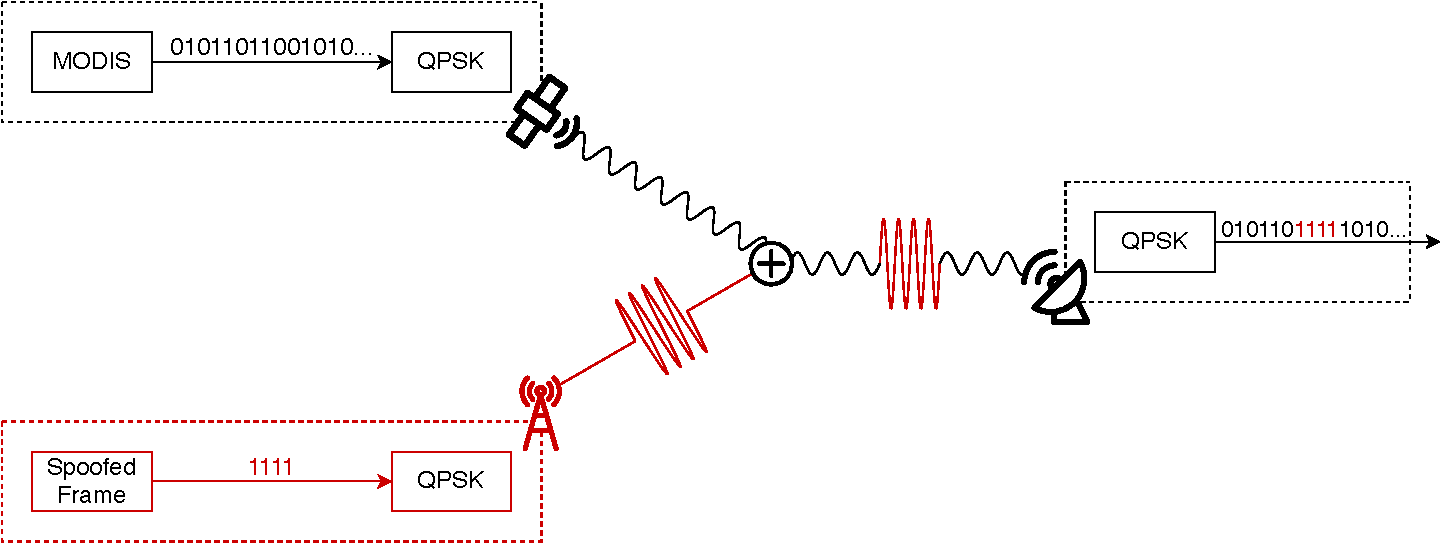
\includegraphics[width=\columnwidth]{diagrams/overshadowing_demo.pdf}
    \caption{Representation of a signal injection attack through overshadowing.}
    \label{fig:overshadowing_demo}
\end{figure}
\end{comment}

\begin{figure}
    \centering
    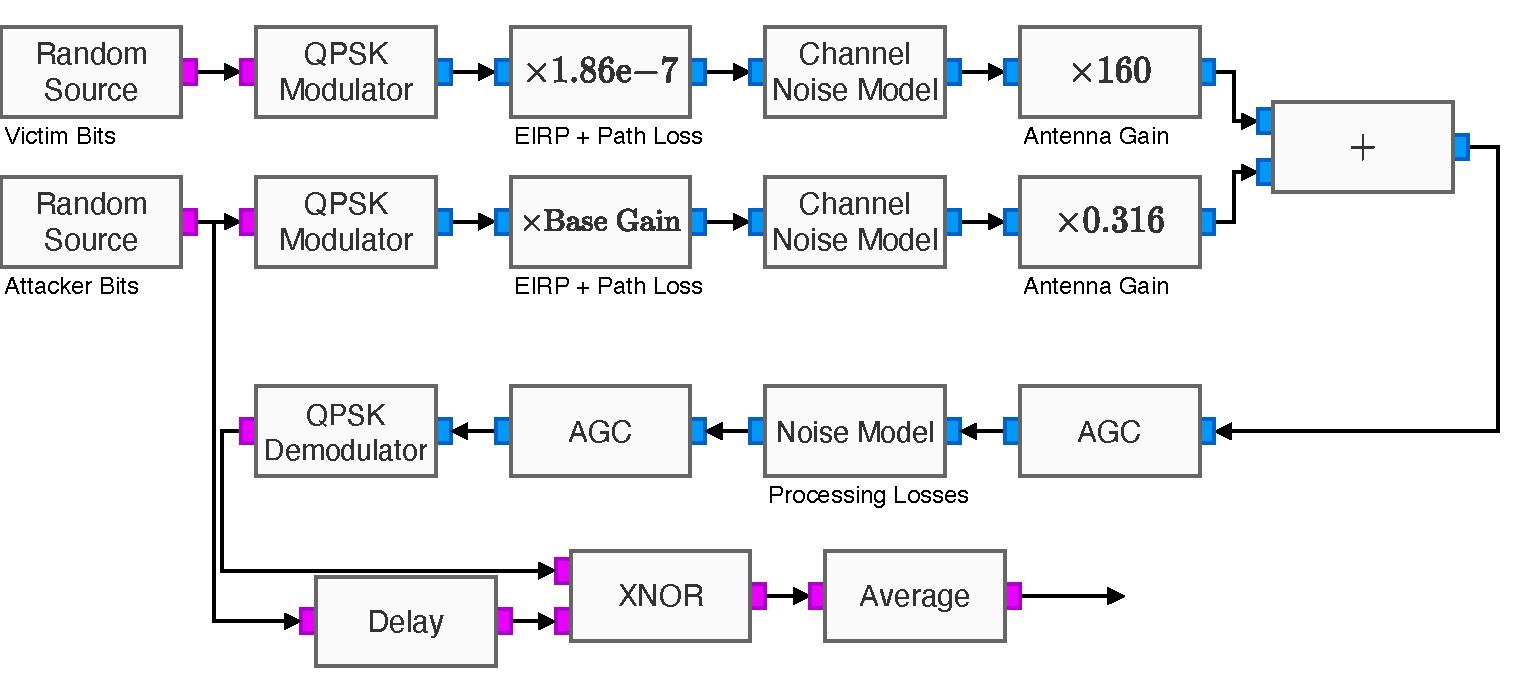
\includegraphics[width=\columnwidth]{diagrams/overshadowing_pipeline.pdf}
    \caption{An overview of the GNU Radio pipeline used to provide experimental validation for the overshadowing attacks. IQ samples are indicated in blue, bitstreams in magenta.}
    \label{fig:overshadowing_pipeline}
\end{figure}

In order to demonstrate the feasibility of signal injection attacks on EOS downlink systems in a real-world setting, we perform a simulated analysis of the proposed attacks.
We use ``GNU Radio'' to construct a pipeline which simulates a legitimate downlink signal broadcast from the Terra satellite and demodulated by a standard QPSK \textbf{TODO make sure explained} demodulator.
We also simulate an attacker-injected signal added to the legitimate signal and demodulated by the same process.
By varying the gain on the injected signal and measuring the Bit Error Rate (BER) of the decoded bytes, we can assess the transmission power required for the attack to succeed.
The concept of signal overshadowing is illustrated in Figure~\textbf{TODO}, and an overview of the experimental configuration is shown in Figure~\ref{fig:overshadowing_pipeline}.
The source code is also available alongside our other artifacts (\textbf{TODO}).

In order to carry out these simulations with a reasonable degree of confidence that they accurately represent the real world, we establish simulation parameters based on known characteristics of the EOS radio systems.
We use the link budget established in~\cite{quinnNew2003} to establish the Effective Isotropic Radiated Power (EIRP) and free-space path loss of the radio signals transmitted by the Aqua and Terra satellites, as well as the antenna gain for signals within the beam of the receiver, and losses within the signal processing pipeline.
We also look at the specification for a commercial EOS ground station to understand how the hardware compares to NASA's ground stations~\cite{dartcomsystemsltdXBand2021}.
On the attacker's side, we use the following standard formula for computing Free-Space Path Loss (FSPL):
\begin{align}
    \text{FSPL}_{\text{dB}} = 20\log_{10}(d) + 20\log_{10}(f) - 147.55, \label{eq:fspl}
\end{align}
where $d$ is the distance from the receiver in meters, and $f$ is the frequency in hertz.
We use the reference antenna radiation pattern given by the International Telecommunication Union in~\cite{itu2022antenna} to estimate the out-of-beam gain of the receiver to be approximately $-10.0$\,dB.
These key values are summarised in Table~\ref{tab:experimental-values}.

\begin{table}
    \resizebox{\columnwidth}{!}{%
    \begin{tabular}{lcc}
        \toprule
        & Victim & Attacker \\
        \midrule
        EIRP (dBm) & $44.4$ & $[0 \dots 100]$ \\
        Distance $d$ (km) & $\sim 713$ & $[0 \dots 10]$ \\
        Free-Space Path Loss (dB) & $179.0$ & $\text{FSPL}_{\text{dB}}(d)$ \\
        Amplitude Multiplier $\left(m = 10^{\frac{\text{EIRP}_{\text{dB}}-\text{FSPL}_{\text{dB}}}{20}}\right)$ & $1.86 \cdot 10^{-7}$ & $m$  \\
        Antenna Gain $g_A$ (dB) & $44.1$ & $-10.0$ \\
        Antenna Amplitude Multiplier $\left( m_A = 10^{\frac{g_A}{20}} \right)$ & $160$ & $0.316$ \\
        System Losses (dB) & $3.7$ & $3.7$ \\
        \bottomrule
    \end{tabular}%
    }
    \caption{Key values used in overshadowing simulations.}
    \label{tab:experimental-values}
\end{table}

We take a range of values for the signal strength at the receiver, between $-100$ and $0$\,dBm.
Received signal strength can be expressed as a function of the attacker's EIRP and distance from the receiver, enabling us to observe the bit error rate as we vary either of these parameters.
We do not accurately model system losses -- since these are consistent between the victim and attacker, we assume their effect on the outcome of the experiment is negligible.
This is verified to be the case by performing the same experiment across a range of noise values and confirming that the result changes by a negligible amount, as seen in Figure~\ref{fig:overshadowing_ber}.
For the main experiments, we set the background noise voltage to $1\,$\textmu V and the system noise to $200$\,mV, resulting in a bit error rate below the $5$\% required for the system to function.

\begin{figure}
    \centering
    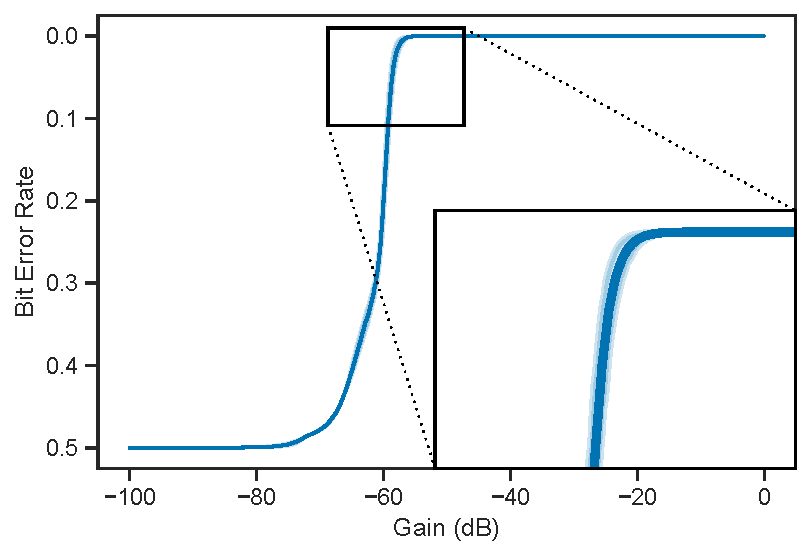
\includegraphics[width=\columnwidth]{diagrams/overshadowing_ber_2.pdf}
    \caption{Error rate of attacker-injected bits as the signal strength at the receiver increases. The small shaded region represents the range of values under different levels of background and system noise.}
    \label{fig:overshadowing_ber}
\end{figure}

The immediate results of our experiment are shown in Figure~\ref{fig:overshadowing_ber}, which compares the signal strength at the receiver to the BER of the injected signal.
In order to understand these results in a meaningful sense, we need to instead consider the factors directly controlled by the attacker: the EIRP of the transmitted signal, and the distance between the attacker and the receiver.
We take the EIRP and subtract FSPL (computed from distance using Equation~\ref{eq:fspl}) to get the received signal strength.

\begin{figure}
    \centering
    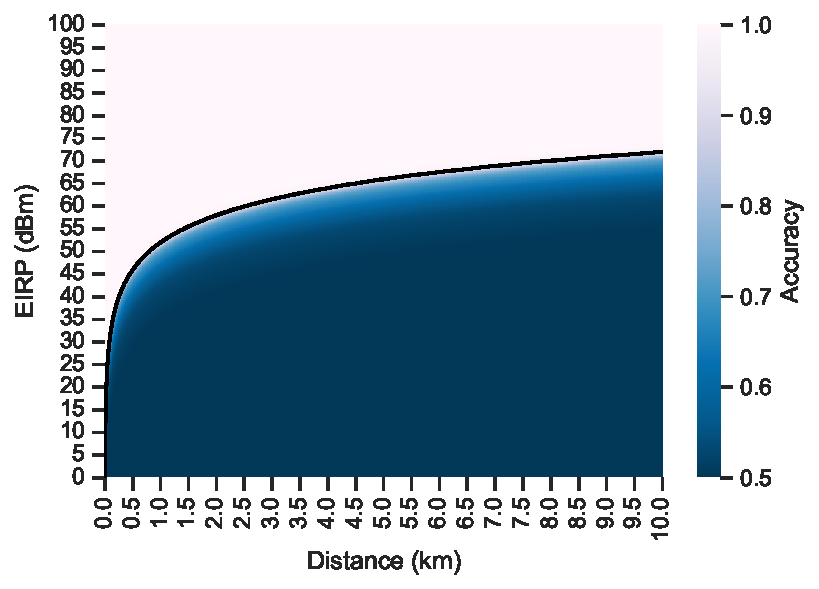
\includegraphics[width=\columnwidth]{diagrams/distance_eirp_heatmap_95.pdf}
    \caption{The bit error rate of the injected signal as the attacker varies EIRP and distance from the receiver. The values beyond which the bit error rate drops below $5$\% are indicated using a line.}
    \label{fig:distance_eirp}
\end{figure}

We see the results in Figure~\ref{fig:distance_eirp}, displaying the BER of the injected signal across a range of EIRPs and distances.
This allows us to better understand the threat model initially established in Section~\ref{sec:threat-model}.
The datasheets for the COTS radio equipment described in this section has an EIRP of up to $49$\,dBm -- we therefore know from our experimental results that an attacker with access to this equipment can carry out overshadowing attacks from a distsance of up to $0.71$\,km~\cite{endurosat:xbandtransmitter,endurosat:xbandantenna}.
With access to a more powerful amplifier, the feasible attack range can be extended significantly; an organized criminal group or nation-state level attacker could reasonably be assumed to have access to these.

We conclude from these results that there is moderate cause for concern regarding overshadowing attacks on NASA ground stations -- a motivated hobbyist with a relatively small budget can carry out attacks from a moderate distance, and attackers with greater means can do so from even further away.
Furthermore, it is difficult to prevent overshadowing attacks without some method of validating the authenticity of the received signal, and locating the attacker requires a specialized setup to triangulate the signal's origin.
This has implications beyond the attacks described in this paper, demonstrating that all downlink processing systems should be regarded as untrusted unless the data link is authenticated in some way.
 % two experiments
\section{Background}\label{sec:background}
\begin{figure}
    \centering
    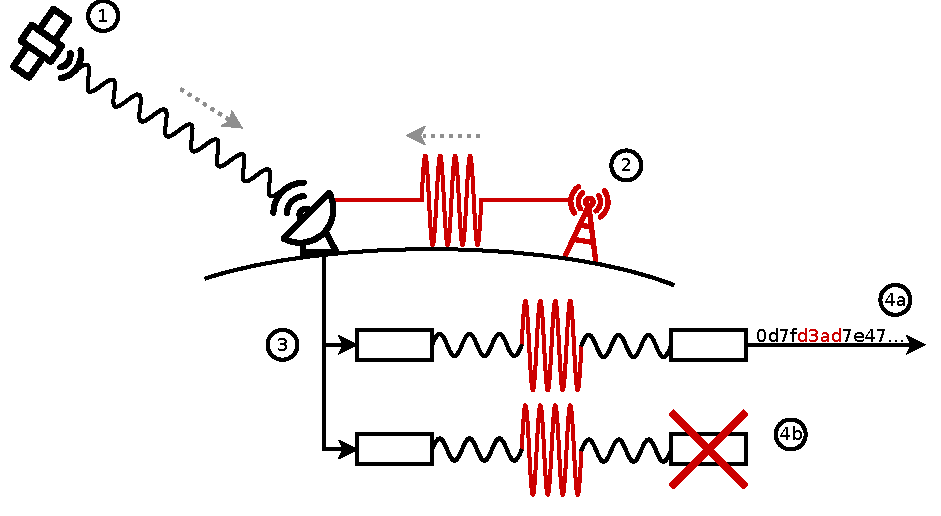
\includegraphics[width=\columnwidth]{diagrams/attack_illustration.pdf}
    \caption{An illustration of the attacks described in this paper. The attacker is indicated in red. 1)~The satellite broadcasts a signal; 2)~A ground-based attacker injects a crafted signal, overshadowing the legitimate signal and resulting in one of two scenarios; 3a)~The victim receiver decodes the attacker-controlled data, poisoning derived datasets; 3b)~The injected signal exploits vulnerabilities in the protocol decoders, resulting in denial of service or arbitrary code execution.}
    \label{fig:attack-illustration}
\end{figure}

Earth observing satellite systems are widely used in a variety of contexts, providing high-resolution images and sensor readings available within hours or less of the initial readings being taken.
Accordingly, a growing market for satellite-derived datasets has emerged which process data for specific purposes including forest fire, dust storm detection, ozone layer depletion, and flooding. \textbf{TODO: make sure these purposes are linked from the table}
Table~\ref{tab:satellite-derived-datasets} summarises a number of currently available satellite-derived datasets, which are derived from a mixture of self-operated, commercial, and open access satellites.

NASA's \textit{Fire Information and Resource Management System} (FIRMS) is one such use case for satellite-derived data, providing a real-time fire notification service which is used for emergency response, disaster planning, and crisis analysis by the fire agencies of over 90 countries. \textbf{TODO: must cite}
FIRMS depends on data derived from the Earth Observing System (EOS) fleet to detect precise locations of fires; an example of a surface image overlaid with detected fires is seen in Figure~\ref{fig:bushfire}.
This is possible because certain satellites in the EOS fleet contain instruments such as the \textit{Moderate Resolution Imaging Spectroradiometer} (MODIS), which provide near real time calibrated light readings across frequency bands wider than the visible spectrum.
The presence of a fire is primarily indicated by high amplitudes in the infrared bands. \textbf{todo: cite MOD14 technical manual}

Specifically, the MODIS instruments are on board \textit{Terra} and \textit{Aqua}, two EOS fleet satellites.
Thanks to their opposite polar sun-synchronous orbits, Terra and Aqua together image the entire surface of the Earth twice per day. \textbf{TODO: fact check}
The data is downlinked to receiver stations across the world in a continuous stream known as \textit{direct broadcast}, or instead as a buffered data dump to a few select locations.
As a result, MODIS data is widely available both from the central NASA archives \textbf{TODO: link} and from any of the 168 alternative receiver stations~\cite{nasaDirect}.

Even though Terra and Aqua were launched in 1999 and 2002 respectively, MODIS-derived datasets continue to see current usage across a wide variety of fields.
The high design specifications and high upfront costs mean that missions tend towards long lifespans, remaining useful for many decades.
For example, MODIS datasets continue to be used to improve fire detection algorithms, and more recently have been used to analyze weather-dispersed diseases that pose serious risks to human health~\cite{valleyFever}.

However, over the last few decades, attitudes towards securing the wireless channel in communications systems have changed significantly.
Previously, overshadowing the signal to inject data or deny service would have required a costly and highly specialized setup; since the advent of the software-defined radio, such attacks now only require access to hardware available off-the-shelf.
It is now commonly known that, using this hardware, attackers can leverage overshadowing to manipulate communications or deny service in areas such as mobile internet~\cite{yang2019hiding,erni2021adaptover}, GNSS~\cite{tippenhauer2011requirements}, and even electric vehicle charging\textbf{TODO: more examples}.
In these cases, the attacker has been enabled by a lack of robust cryptography in the systems being faced. % TODO: rephrase

% TODO: insert diagram of common space comms protocols
% TODO: find out which other satellites are unencrypted, and especially those which are new and use CCSDS
% Are they generally encrypted above the CCSDS layer?

Many Earth observing satellites face similar issues, since these systems were built at a time when robust cryptography was uncommon due to less powerful onboard computers.
Therefore, while it is unsurprising that such systems are not resilient against modern adversaries, it is surprising that safety-critical infrastructure depends upon the resulting data.
These satellites include NASA's Earth Observing Fleet and NOAA's GOES fleet, which provide no cryptographic authenticity guarantees.
They also include satellites which only implement partial or now-insecure cryptography, or those whose keys have been leaked.

% TODO: summary paragraph of these
For example, the Korean satellite COMS-1 uses single DES encryption~\cite{lrit-key-dec}, which has led to its keys being successfully extracted from satellite data. \textbf{TODO: confirm this is an accurate summary from the blog post, which seems to imply that a server was involved}
Additionally, GEO-KOMPSAT-2A had its keys leaked on the Korea Meteorological Administration website, and to this day remain publicly available~\cite{xrit-rx}.
We should continue to expect that more encrypted satellite communications become publicly decryptable, as once-secure encryption standards and practises result in leaked encryption keys, some of which will be irrevocably baked into the firmware.

Due to the constraints of the time and a desire to make the data open access, Terra and Aqua downlink their data in the clear.
Therefore, modern off-the-shelf radio hardware enables attackers to overshadow and manipulate the raw data.
This can result in derived datasets poisoned with false information, with the processing pipeline stages themselves also potentially exploitable.

We proceed to precisely define the nature of the threat in Section~\ref{sec:threat-model}.
Using FIRMS as a case study, we describe how the attacker can poison the derived datasets and exploit the processing stages in section~\ref{sec:attack}.
We demonstrate that overshadowing the physical layer is sufficient to arbitrarily manipulate the fire detection algorithm, and achieve denial of service and code execution on the processing software.
We go on to validate the feasibility of the overshadowing approach in Section~\ref{sec:evaluation}, considering the case of a terrestrial attacker against a highly directional dish.

\begin{figure}
    \centering
    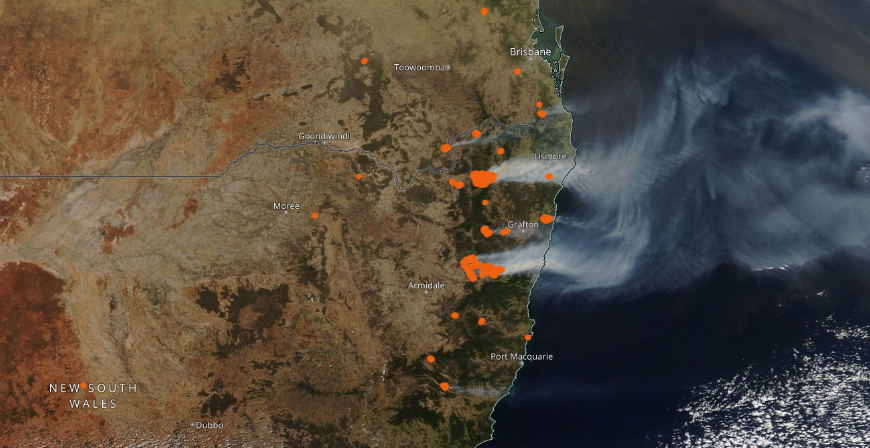
\includegraphics[width=\columnwidth]{diagrams/bushfire.png}
    \caption{The 2019 Australia bushfires as seen from Aqua's MODIS instrument, annotated with the \textit{Fires and Thermal Anomalies} dataset on NASA's worldview.\protect\footnotemark}
    \label{fig:bushfire}
\end{figure}

\footnotetext{Image taken from \url{https://worldview.earthdata.nasa.gov/?v=138.5214305912576,-37.663755528187544,165.90196079866635,-23.47436617591061\&as=2019-09-07-T00\%3A00\%3A00Z\&ae=2019-10-26-T16\%3A00\%3A00Z\&l=MODIS\_Combined\_Thermal\_Anomalies\_All,VIIRS\_SNPP\_Thermal\_Anomalies\_375m\_Day(hidden),VIIRS\_SNPP\_Thermal\_Anomalies\_375m\_Night(hidden),Reference\_Labels\_15m,Reference\_Features\_15m,Coastlines\_15m,VIIRS\_SNPP\_CorrectedReflectance\_TrueColor(hidden),MODIS\_Aqua\_CorrectedReflectance\_TrueColor,MODIS\_Terra\_CorrectedReflectance\_TrueColor(hidden)\&lg=false\&al=true\&av=3.5\&ab=on\&t=2019-09-07-T02\%3A00\%3A00Z}}


% TODO: add info about Google Maps
\begin{table*}
    \resizebox{\textwidth}{!}{%
    \begin{tabular}{lllll}
        \toprule
                     &       & \multicolumn{2}{c}{Satellites} & \\
        \cmidrule(lr){3-4}
        Organization & Usage & Provider & Nature & Data Access \\
        \midrule
        Planet Labs~\cite{planetProducts} & Various (intelligence, infrastructure, & Planet Labs & Self-operated & Commercial \\
                    & land use, water use) & & & \\
        Global Forest Watch~\cite{gfwMap} & Forest monitoring, carbon use, deforestation & Planet Labs & Commercial & Open access \\
        California Forest Observatory~\cite{cfoMap} & Monitoring forest fires in California & Planet Labs & Commercial & Open access \\
        ESRI~\cite{esriMap} & Land-use and land-cover maps & ESA (Sentinel-2) & Open access & Open access \\
        %Salo Sciences (TODO only bring back if I can say something about "forest restoration monitoring" project) & Conservation, climate monitoring & Planet Labs & Commercial & \\
        Meta~\cite{metaMap} & Population density maps & DigitalGlobe & Commercial & Open access \\
        Cloud to Street~\cite{cloudToStreet} & Flood tracking (disasters and insurance) & NASA (Terra/Aqua) & Open access & Commercial \\
        NCX Basemap~\cite{ncxBasemap} & Timber and carbon value monitoring in the USA & NASA & Open access & Commercial \\
        Upstream Tech HydroForecast~\cite{hydroforecast} & Water flow and weather intelligence & NASA (Terra/Aqua) & Open access & Commercial \\
        NASA FIRMS~\cite{nasaFirms} & Fire detection and management & NASA (EOS) & Self-operated & Open access \\
        \bottomrule
    \end{tabular}
    }
    \caption{Information on a number of satellite-derived datasets, including the satellite providers used to source the data.}
    \label{tab:satellite-derived-datasets}
\end{table*}


\subsection{Related Work}

% TODO: GNSS spoofing - mention in related work?
% https://www.usenix.org/conference/usenixsecurity19/presentation/yang-hojoon\textbf{TODO write}
%
\begin{itemize}
    \item existing work in signal spoofing, signal sniffing, possibly other attacks, possibly draw parallels with ads-b
    \item existing work in satellite security, countermeasures to this stuff
    \item explain how our work is novel and builds on these
\end{itemize}

Our work builds on \textbf{TODO}

Existing work within the field of satellite security focuses on either \textbf{TODO spoofing GPS-like signals or sniffing communications}
In 2020 it was demonstrated that confidential maritime satellite communications could be received by an SDR-equipped attacker from a great distance away (covering a total area of tens of millions of square kilometers), thanks to the satellites' wide beamwidth and unencrypted payload~\cite{pavurTale2020}.
This work also explores the theoretical possibilities of TCP session hijacking by broadcasting signals over a high-speed wired connection.
Our work differs in this respect -- we focus on the vulnerabilities created by an attacker capable of injecting signals over the radio link, compromising trust in the received signal.

In~\cite{wuSpoofing2020} we see a comprehensive review of spoofing and jamming attacks against GNSS (positioning and navigation) satellites, resulting in denial of service and incorrectly reported positions respectively.
Spoofing attacks are carried out by replay, forgery, and other methods to fool the receiver.
This work also includes a review of methods by which spoofing and jamming can be detected or mitigated.
These methods include consistency checking, measuring signal characteristics, measuring arrival times, utilizing arrays of antennas, measuring angle of signal arrival, and a number of other techniques.
We apply some of these concepts to the novel threat model presented by \textbf{TODO}; we demonstrate that signal spoofing is possible for satellites for which the receiving and broadcasting equipment was previously thought to make such attacks prohibitively expensive, and show that attacks can have a significant effect on processing systems downstream from the original data.
We also explore in Section~\ref{sec:countermeasures} how an existing system might apply novel and already known countermeasures to existing systems to reduce the attack surface.

There is also work showing that it is possible to spoof satellite signals, particularly when not encrypted; \textbf{TODO} demonstrates this using the GPS positioning satellites.
By exploiting the unauthenticated nature of the signals it is possible to modify the unauthenticated data; our work builds on this by demonstrating that this is also possible for satellites for which the receiving and broadcasting equipment was previously thought to make such attacks prohibitively expensive.
We also look beyond the payload and look at attacks on the data processing system itself to create novel attacks.

\textbf{TODO something about packet-based broadcast vs continuous broadcast?}

There is also wider work in the security community surrounding signal spoofing and its detection -- for instance, Čapkun et al.\ detect GPS spoofing by observing the physical properties of the signal alongside inspecting downlinked data \textbf{TODO cite SPREE}.
\textbf{TODO more?}
We \textbf{TODO}.


% To go in the attack description:
\begin{comment}
The data is downlinked in almost exactly the same format for both the main data dump and the direct broadcast.
Packets from the MODIS instrument are encapsulated wthin the CCSDS Space Packet Protocol (SPP), which are packed within an unencrypted custom data link protocol known as the \textit{Channel Access Data Unit}, or CADU.
Finally, the CADUs are modulated using \textit{Quadrature Phase Shift Keying} (QPSK) and transmitted on the X-band, centered at 8160\,MHz. \textbf{TODO: is this the same for both DB and TDRSS dump?}

% TODO: is such an in-depth explanation required here?
The raw SPP packet data is known as \textit{Level 0}, and is processed through a chain of programs distributed through the IPOPP framework to generate higher-level satellite-derived datasets.
The other EOS fleet satellites are processed in much the same way.
The Level 0 data is processed into \textit{Level 1}: an easier to use heirarchical data format, optionally geolocated to a subpixel accuracy using timing information, the satellite's orbital parameters, and an accurate model of the Earth's surface.
Level 1 data is processed into a variety of \textit{Level 2} datasets, including fire detection, land surface temperature values, vegetation detection, etc.
Finally, certain Level 3 datasets are produced, which generally consist of composites of the Level 2 data for specific purposes, such as analysing post-fire burned areas.
\end{comment}

% Tasked vs untasked images - aka when you have to ask to point the satellite, vs it just gets everything
 % describe the related work
\section{Countermeasures}\label{sec:countermeasures}

Fundamentally, the attacks described in this paper arise from a lack of caution towards input data -- it is assumed that all incident signals on the receiver are legitimate, well-intentioned, and safe to process.
Under these assumptions, it makes sense to run all received signals through a processing pipeline which does not handle input data with utmost caution.
However, we have shown in this paper that such assumptions do not hold and a sufficiently motivated attacker with access to common radio hardware can inject crafted signals to cause unwanted behaviour on the target system, compromising data and potentially leading to real-world harms.
\textbf{TODO make sure real-world harms are talked about earlier on}

It is therefore of great importance that input data is handled carefully, and the systems processing such data are protected against known attacks.
There are a few potential methods to achieve these goals:

\subsection{Encryption, Signatures}

One of the most straightforward solutions to suggest would be to simply encrypt the downlinked signals using a key known only to the operators.
While this may seem simple, there are a number of reasons not to take this approach: although it may seem that it would only require a simple software update, the hardware on these satellites is highly specialised and it may be a challenge to insert encryption into the radio downlink pipeline.
Satellite hardware is also computationally limited due to the requirement of high levels of radiation shielding and error correction, so it may not be feasible to perform the computation required for encryption onboard.

Even if these problems can be resolved, encrypting signals from the EOS fleet would be detrimental to a large number of businesses and research institutions which have set up their own ground stations to receive downlinked signals.
These parties would no longer be able to receive signals, rendering their often expensive ground stations worthless. \textbf{TODO: We can't claim this, since signatures are a cryptographic primitive that keeps data publicly available}
This problem could be sidestepped by instead signing the data using a cryptographic key, but this would still likely require significant changes to the signal processing pipelines in use by these organisations.

\subsection{Placeholder}
\textbf{TODO think of title here}

A more straightforward approach is for the receiving ground stations to simply treat downlinked data as untrustworthy, and build software and hardware stacks accordingly.
Such behaviour includes keeping all software and libraries used in data processing fully up-to-date in order to reduce the threat of known vulnerabilities, as well as making sure input data is properly sanitised before passing into other tools/libraries or running shell commands derived from the input.

This is helped by making sure processing software is not bloated and does not pull in excessive dependencies, and that the code written is well-documented and easy to understand, maintain, and update.

\section{Conclusion}

Having demonstrated the impact of signal injection attacks on systems which assume input data to be safe, a discussion remains to be had on how this situation was reached in the first place.
Fundamentally, the assumption that all input data is safe led to a lack of safety checks and input sanitization in the pipeline, allowing any data to be processed, including that which was crafted by an attacker.
This is compounded by a lack of security in bundled dependencies -- the system contains many redundant dependencies, including ones years out of date.
This opens the system up to a huge number of known vulnerabilities which could be mitigated simply by using the latest versions of dependencies which have patched known security holes.

However, another core problem in this processing system is a lack of transparency within the codebase itself, making simple security audits and updates nearly impossible.
The system is also brittle, with a number of potential exploits currently prevented by minor variables or configurations -- if these were to change in an update the system could easily become far more vulnerable.
A redesign of this system could simplify the flow of data through it and make it far easier to understand and maintain, which would in turn make it far more secure.

\textbf{TODO wrap this up nicely, probably rewrite earlier bits as well}


\newpage
% Fix repeated authors showing as dash
\bstctlcite{IEEEexample:BSTcontrol}

\bibliographystyle{IEEEtranS}
\bibliography{IEEEabrv,refs}
\end{document}
